\section{APPENDIX}
\noindent
\rule{7.0in}{.013in}

\begin{center}
	\subsection{Spectrogram Examples}\label{appx:spectra}
\end{center}

As produced by the \verb+Spectrogram+ class.

\begin{figure}[h]
	\centering
	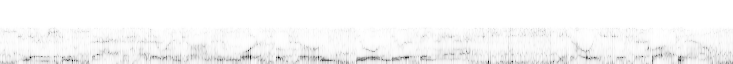
\includegraphics[width=500pt]{../graphics/lpc_spectrograms/ian15_wav.png}
	\caption{LPC spectrogram obtained for ian15.wav}
	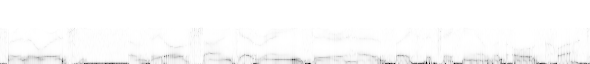
\includegraphics[width=500pt]{../graphics/lpc_spectrograms/graham13_wav.png}
	\caption{LPC spectrogram obtained for graham13.wav}
\end{figure}

\begin{center}
	\subsection{MARF Source Code}
\end{center}

You can download
the code from \verb+<http://marf.sourceforge.net>+, specifically:

\begin{itemize}
\item The latest unstable version: \verb+<http://marf.sourceforge.net/marf.tar.gz>+
\item Browse code and revision history online: \verb+<http://cvs.sourceforge.net/cgi-bin/viewcvs.cgi/marf/>+
\end{itemize}

API documentation in the HTML format can be found in the documentation
distribution, or for the latest version please consult:
\verb+<http://marf.sourceforge.net/api/>+. If you want to participate
in developement, there is a developers version of the API:
\verb+<http://marf.sourceforge.net/api-dev/>+, which includes
all the private constructs into the docs as well.

\clearpage

\begin{center}
	\subsection{SpeakerIdentApp and SpeakersIdentDb Source Code}
\end{center}

\subsubsection{SpeakerIdentApp.java}

\vspace{15pt}
\hrule
{\scriptsize \input{SpeakerIdentApp}}
\hrule
\vspace{15pt}

\subsubsection{SpeakersIdentDb.java}

\vspace{15pt}
\hrule
{\scriptsize \input{SpeakersIdentDb}}
\hrule
\vspace{15pt}

\clearpage

\begin{center}
	\subsection{TODO}\label{appx:todo}
\end{center}

\vspace{15pt}
\hrule
{\scriptsize \input{TODO}}
\hrule
\vspace{15pt}
